\documentclass[journal,10pt,twocolumn]{article}
\usepackage{graphicx, float}
\usepackage[margin=0.5in]{geometry}
\usepackage{amsmath, bm}
\usepackage{array}
\usepackage{booktabs}
\usepackage{mathtools}

\providecommand{\norm}[1]{\left\lVert#1\right\rVert}
\let\vec\mathbf
\newcommand{\myvec}[1]{\ensuremath{\begin{pmatrix}#1\end{pmatrix}}}
\newcommand{\mydet}[1]{\ensuremath{\begin{vmatrix}#1\end{vmatrix}}}

\title{\textbf{Optimization Assignment}}
\author{K prathyusha }
%\date{September 2022}

\begin{document}

\maketitle
\paragraph{\textit{Problem Statement} -Find the maximum and minimum values of $x+sin2x$ on (0,2$\pi$).}

\section*{\large Figure}

\begin{figure}[H]
\centering
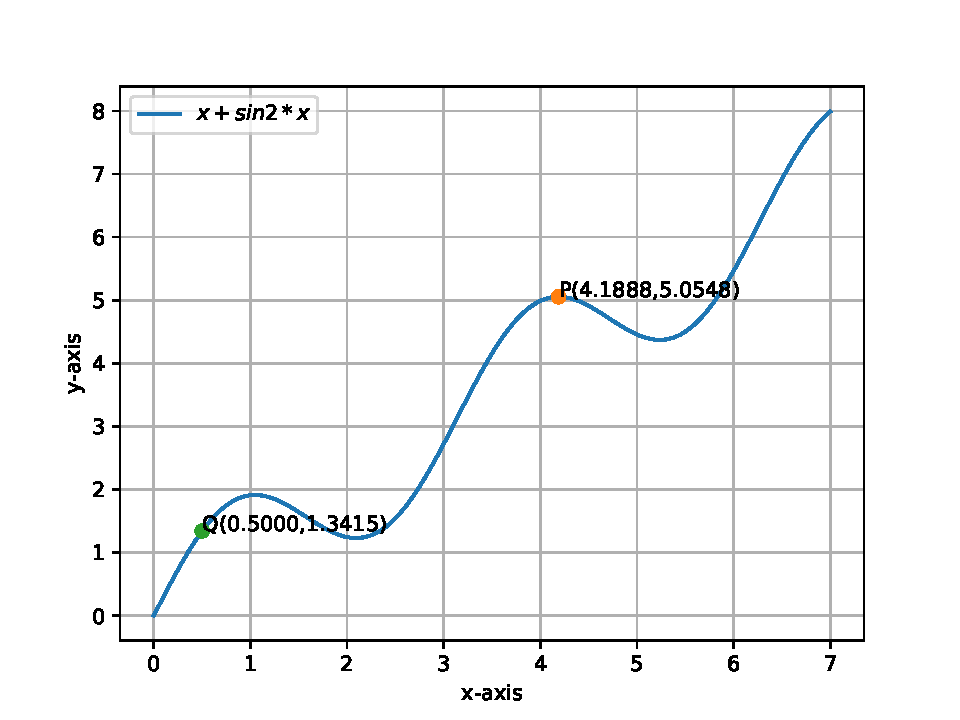
\includegraphics[width=1\columnwidth]{/sdcard/Download/fwc/optimization/opt.pdf}
\caption{Graph of f(x)}
\label{fig:triangle}
\end{figure}
\section*{\large Solution}

	
    \subsection*{\normalsize Gradient descent}
    
    
    \begin{align}
	\label{eq:vol_varx}
	f(x) = x+sin2x\\
    f'(x) = 1+2cos2x
	\end{align}

we have to attain the maximum and minimum values of x+sin2x in the interval [0,2$\pi$]. This can be seen in Figure f(x).Using gradient ascent method we can find its maxima and minima in the interval [0,2$\pi$]
\begin{equation}
        x_{n+1} = x_n + \alpha \nabla f(x_n) 
\end{equation}
\begin{equation}
	x_{n-1} = x_n - \alpha \nabla f(x_n)  
\end{equation}
\vspace{1mm}
\begin{equation}
\implies x_{n+1}=x_n+\alpha(1+2cos2x)
\end{equation}
\begin{equation}
\implies x_{n-1}=x_n-\alpha(1+2cos2x)
\end{equation}
Taking $x_0=0.5,\alpha=0.001$ and precision = 0.00000001, values obtained using python are:
    

    \begin{align}
        \boxed{\text{Maxima} = 1.0472}\\
        \boxed{\text{Maxima Point} = 1.9132} \\
	\boxed{\text{Minima} = 0.5000} \\
	\boxed{\text{Minima Point} = 1.3415}
    \end{align}
   
    

    





 






\end{document}
